\chapter{Game Tags for Visual Video Seach}\label{chap:ecir}

\begin{quotation}
\noindent
In this chapter we start investigating the usefulness of the user tags for search. Throughout this thesis we will address two prominent search scenarios that arise in practice. The first scenario is retrieving video fragments that feature \textit{visual appearances} of objects. In fact, this is very much like the instance search task from TRECVID\footnote{\url{http://trecvid.nist.gov/}} with the difference that query is formulated in text and not by visual example as in TRECVID. The second scenario we consider is topical search i.e. retrieval of video fragments that are about a given topic. In this chapter we study how effective are the user tags in the addressing the first scenario. The methodology that we use is \textit{quantitative system evaluation} \cite{vorhees}. In order to evaluate effectiveness of information retrieval, this methodology requires collection of ``documents'' (in our case video fragments tagged by users via \textit{Waisda?}), set of queries which we derived from real-life query logs, and relevance judgments  indicating which ``documents'' in the collection should be returned for each query. The query set that is created in this chapter is reused in the subsequent Chapter \ref{chap:topicir-filter}, where we address the second scenario.

This chapter was published as ``An Evaluation of Labelling-Game Data for Video Retrieval" in the proceedings of the European Conference of Information Retrieval 2013 \cite{ecir}. It was co-authored with Michiel Hildebrand, Jacco van Ossenbruggen, Lora Aroyo, and Guus Schreiber.
\end{quotation}

\section{Introduction}\label{sec:intro}

Games with a purpose are a way to make humans solve tasks in an entertaining setting. Video tagging games ---a type or GWAPs---	
% is one of the tasks that is being outsourced to internet users. 
%Harnessing users' efforts to amass video annotations 
could become an attractive alternative (or enhancement) to professional annotators in terms of both price and scale. While user tags are virtually for free and plentiful, professional annotations are costly and scarce.
% Consequently, increasing number of video collection owners are deploying GWAPs to collect user tags for their video material. For example,
The Institute for Sound and Vision (S\&V)\footnote{S\&V, \url{http://www.beeldengeluid.nl/}, is the Netherlands national archive.} launched \textit{Waisda?}\footnote{At the time of writing, \textit{Waisda?} is an ongoing project for three years and the game has seen its second release, \url{http://woordentikkertje.manbijthond.nl/}.}, a multi-player video labelling game where players describe streaming video by entering tags and score points based on temporal tag agreement.  The underlying assumption is that tags are faithful descriptions of the videos when entered independently by at least two players within a given time-frame.  From here on we shall refer to such mutually agreed upon tags as \textit{verified} tags.

The archive expects that tags collected with \textit{Waisda?} will improve video search. In this study, we put this hypothesis to the test.
Knowing that other types of video metadata will also be present, our first research question is:
\begin{itemize}
\item[RQ1] Can user tags, on their own or in combination with other types of metatada, improve video search?
\end{itemize}
To test the assumption that agreement is a good filter,  our second research question is:
\begin{itemize}
\item[RQ2] Does limiting only to verified user tags gives better video search performance than considering all user tags?
\end{itemize}
%\textit{RQ3: Which types of video search queries benefit from exploiting user tags?}\\
When GWAPs are used to tag large video collections generally care must be taken to ensure `fair' distribution of game-time across the collection items. In this sense it is instructive for collection administrators and scheduling algorithms designers to know if search performance deteriorates or stagnates after certain point, or if more tags always give better search performance. Therefore, our last research question deals with search performance change over time:
\begin{itemize}
\item[RQ3] How does the user tag search performance change when tags are added?
\end{itemize}

The rest of the paper is structured as follows.  After discussing related work, Sect. \ref{sec:approach} presents our approach. 
Section \ref{sec:materials} describes the datasets and resources that are used in our study. 
%Section \ref{sec:eval-dataset} outlines our evaluation dataset. 
Section \ref{sec:experimental-setup} introduces the experimental setup. Finally, Sect. \ref{sec:results} and \ref{sec:conclusions} present the results and conclusions of this study, respectively.

\section{Related Work}\label{sec:related-work}
\paragraph{User annotations for video.}Video annotation is a tedious and time-consuming activity. Not surprisingly, various initiatives exist that aim at collecting video annotations through crowdsourcing. In particular, \textit{LabelMe video} is an online video annotation system that allows users to identify objects and annotate visual features such as motion and shapes \cite{labelme}. However, this frame-by-frame conceptually low-level annotation remains a tedious task. The willingness of people to participate without compensation is limited at best. To alleviate this, \cite{turk1,turk2} employ the crowdsourcing MTurk platform to recruit annotators which are paid for the task. An alternative way to motivate people is to gamify the annotation experience through GWAPs. GWAPs are computer games, in which people, as a side effect of playing, perform tasks computers are unable to perform. The main example of a GWAP is Luis von Ahn's ESP image labeling game \cite{CHI2004:vonAhn}. Evaluation shows that these labels can be used to retrieve images with high precision and are almost all considered as good descriptions in a manual assessment. The idea to annotate through GWAP has been applied to video in, for example, the Yahoo! video tag game \cite{WWW08_vanZwol_etal}, VideoTag\footnote{\url{http://www.videotag.co.uk/}} , PopVideo\footnote{\url{http://www.gwap.com/gwap/gamesPreview/popvideo/}} and \textit{Waisda?}. With some slight differences, in each of these games players describe streaming video by assigning free-text tags. Thus, we deem \textit{Waisda?} as a typical representative of video GWAPs. 
%What distinguishes \textit{Waisda?} from the other video labelling games is the fact that it was deployed by S\&V with the intention of collecting metadata for improving access to their collection. In this work we study to what extend this is achieved.
\paragraph{Relevance judgements and search.}Designing ground truth in the form of document relevance w.r.t. a given topic has been playing a central role ever since Cranfield experiments gained prominence\cite{vorhees}. The leading actor in IR benchmarking is TREC\footnote{\url{http://trec.nist.gov/}} which employs substantial manpower in creating the ground truth. For organizations lacking the manpower, crowdsourcing is an alternative; \cite{rjturk1,rjturk2} showed that this task can be reliably fulfilled by crowd workers. Alternatively, Eickhoff et al. gamified the task resulting in increased reliability and reduced cost \cite{rjgame}. In this study we also rely on the crowd; the relevance assessment is outsourced to targeted fan groups.\\
Search based on user-generated metadata, in particular folksonomies, has been studied before. Morrison compared the search performance of folksonomies from social bookmarking web sites against search engines and subject directories \cite{morison}, showing that search engines had the highest precision and recall rates. Folksonomies, however, performed surprisingly well. Geisler and Burns state that YouTube tags provide added value for search, because 66\% of them do not appear in  other metadata \cite{youtube}. Hildebrand et al. proposed and investigated a semi-automatic process of assigning explicit meaning to user tags for video by linking them to concepts from the Linked Open Data cloud \cite{michiel}. To the best of our knowledge, no work has been done to evaluate the performance of GWAP data for video search. Our study aims to fill this void.

\section{Approach}\label{sec:approach}
In order to assess the added value of user tags for video search we use a quantitative system evaluation methodology \cite{vorhees}, for which we need a document collection (in our setting video fragments tagged by users in \textit{Waisda?}), a set of representative queries, and relevance judgements.
% System evaluation requires collection of ``documents" (in our case video fragments), set of queries, and relevance judgements indicating which ``documents" in the collection should be returned for each query. 
%For this study we create our own evaluation dataset. Alternatively, we could have used one provided by the various video retrieval evaluation initiatives like TRECVID\footnote{\url{http://trecvid.nist.gov/}}. However, \textit{Waisda?}-like games have not been run yet on these datasets and setting up such a game and attracting sufficient number of users could turn out to be a challenge.
We created this evaluation dataset as follows: (i) select a collection of video fragments tagged by players in \textit{Waisda?}, (ii) select a set of user queries from real-life query logs, and (iii) create relevance judgements. All these steps are described in more detail in Sect. \ref{sec:fragment-collection}.
The dataset is then used in two experiments. In the first, we compare performance of search based on different types of metadata. On high-level the work-flow for the experiment is as follows. We create a number of systems (search engines), run them against the evaluation dataset and compute retrieval performance metrics to assess the search effectiveness of the systems. The structure of all systems is the same: each system uses the same state-of-the-art probabilistic ranking function BM25 \cite{bm25}, but indexes pairwise different combinations of metadata types. Thus, the only variations among the systems within an experiment is the input that they exploit for search. In our experiments we built the systems using the Xapian open source search engine library \footnote{\url{http://xapian.org/}}. We did not vary the parameters for the BM25 function and used the defaults provided by Xapian\footnote{The default parameters for the BM25 algorithm are outlined at \url{http://xapian.org/docs/bm25.html}}. The combinations of metadata types that are indexed by the various systems are strategically chosen so that the resulting performance metrics from the benchmarks will provide answers to the research questions. For example, to determine whether we are better off using all tags opposed to only using verified tags ---remember this is the second research question--- for search, in the first experiment we have a system that indexes \textit{all} user tags and a system that indexes \textit{only the verified} user tags. Since the only difference between these two systems is the metadata they use as input for search, any difference between the search performances will stem solely from the metadata. In other words, by comparing the performance metrics of the two systems we can deduce whether using all tags for search is better than using only the matched ones. To get a better idea of what goes wrong when searching using user tags, we also carry out a follow up analysis of a sample of the results deemed as false positives.
In the second experiment, we study the search performance of user tags over time. To this end, we again create a number of systems, but this time each system indexes a weekly snapshots of all tags. Comparing the performances of the systems that index consecutive weekly snapshots reveals how the tag search performance varies over time.

% The first experiment, described in Section \ref{sec:experiment1-setup}, addresses the first two research questions and the second experiment, presented in Section \ref{sec:experiment2-setup}, addresses the third research question. In both experiments, we create a number of systems (search engines), run them against our evaluation dataset, and compute retrieval performance metrics to assess their performance. All systems use the same state-of-the-art probabilistic ranking function BM25 \cite{bm25} and the only variation among them is the metadata that they index. This way differences in performance can be attributed exclusively to the metadata. Besides the user tags, we exploit the following types of metadata: (i) the existing collection metadata in a form of tags and textual descriptions, and (ii) subtitles (closed captions) associated with the videos. Detailed description of the different metadata types is provided in Section \ref{sec:video-metadata}.

\section{Datasets and Resources}\label{sec:materials}
In this section we describe the datasets and resources that are used in the study.
\subsection{The MBH Video and Metadata Collection}\label{sec:video-metadata-collection}
At the time of writing, \textit{Waisda?} is used to % is in its second release. In this release the collection of fragments that are tagged by players originates from 
tag fragments from the popular Dutch TV program `Man Bijt Hond' (MBH) produced by the Dutch broadcaster NCRV.  MBH is a humoristic TV show that focuses on trivial, everyday news and ordinary and unknown people.  Every episode consists of 7-8 unrelated, self-contained fragments where each fragment topically comes under a recurring heading\footnote{The complete list of the recurring headings (categories) can be found at \url{http://www.manbijthond.nl/rubrieken}. Note that at the time of writing the webpage is in Dutch only.}. Players in \textit{Waisda?} tag these fragments.  The entire collection to which we have access has 11,109 fragments from episodes aired in the last 11 years.

%\begin{table}[tb]
%\centering
%\begin{footnotesize}
%\caption{Descriptive statistics for various video metadata types. Note that \# stands for number. The statistics for the user tags are computed on the subset of 2,192 fragments for which there is at least one user tag and the statistics for the NCRV are computed on the entire collection of 11,109 fragments.}
%\begin{tabular*}{\columnwidth}{@{\extracolsep{\fill}}l|rrr}
%\toprule
%& \textbf{All tags} & \textbf{Verified}&\textbf{NCRV tags} \\  
%\midrule
%\textbf{\# of tags}\B \T &436,456  & 243,352&125,137\\
%\textbf{\# of unique tags}\B &47,455  &12,861  & 25,760\\
%\textbf{avg. \# of tags per video}\B& 199 &111& 11.4\\
%\textbf{min. of \# of tags per video}\B&1 &2&1\\
%\textbf{max. of \# of tags per video}\B&3,700 &3147&105\\
%\textbf{median of \# of tags per video}\B&65 &76&11\\
%\bottomrule
%\end{tabular*}
%\end{footnotesize}
%\label{table:tags-stats}
%\end{table}

% \subsection{Video metadata}\label{sec:video-metadata}

In addition to the video fragments, we have access to four types of descriptive metadata that are used as input for search:
\paragraph{\textbf{Waisda? tags.}} We consider the collection of all user tags acquired with \textit{Waisda?} during the first five months, starting from October, 2011. In this period 436,456 different tag entries were assigned to 2,192 video fragments by roughly 24,000 players. The number of unique user tags exceeds 47,000. Each tag entry is associated with the point in time --- relative to the beginning of the fragment --- when the tag was entered. Additionally, each tag entry is marked as `verified' or not based on the tag agreement in its temporal neighbourhood.
%In particular, a tag is verified if it is entered by at least two distinct players in a time interval of 10 seconds.
As the game is advertised only in Dutch media and the material being tagged is exclusively in Dutch, the language of almost all tags is Dutch. The average number of tags per video is 199. Approximately 55\% of all user tags ($\approx$ 243,000) are `verified' and the number of unique verified tags is 12,861. The average number of verified tags per video is 111.
\paragraph{\textbf{NCRV tags.}} NCRV, the broadcaster, maintains an in-house collection of tags % that describe their video material. The purpose of these tags is 
to facilitate web access to MBH fragments via search and browsing. In contrast with \textit{Waisda?} tags, NCRV tags are not time-based, meaning they are not linked to a particular time-point in the video, and generally cover only the prevalent topics. The average number of NCRV tags per video is 11. Thus they are usually much scarcer than the game tags.
\paragraph{\textbf{NCRV catalogue data}.} Along with the curated NCRV tags, each MBH fragment has a short textual description, usually one paragraph, and a title. We consider the collection of all titles and textual descriptions (i.e. catalogue data) as another metadata type that will be used in the study.
\paragraph{\textbf{Captions}.} % Yet another metadata type we make use of is the subtitle files associated with the video fragments. 
Closed captions are textual versions of the dialogue in films and television programs for the hearing impaired, usually displayed at the bottom of the screen. Each dialogue excerpt is accompanied with time-points --- relative to the beginning of the video --- when the dialogue excerpt appears on and disappears from the screen. We use captions  obtained from S\&V\ that cover most of the MBH episodes aired in 2010 and 2011 which amounts to a total of 897 fragments. 

\begin{figure}[t]
\centering
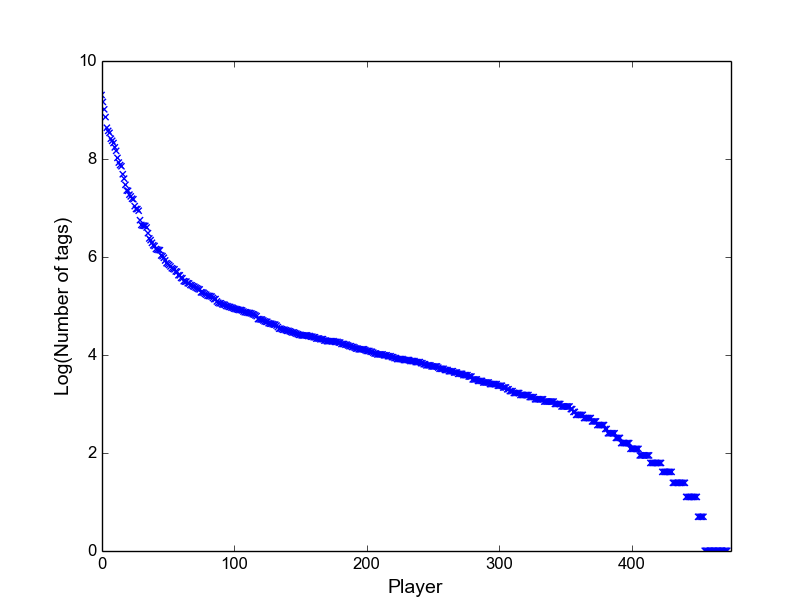
\includegraphics[scale=.4]{ecirnumtagsperplayer} 
\caption{Number of tags contributed by each of the players in the selected sample of fragments. The horizontal axis represents the players ordered decreasingly on the number of tags they entered. The vertical axis displays the logarithm to base 2 of the number of tags entered by the associated player.}
\label{numtagsperplayer}
\end{figure}

\subsection{Evaluation Dataset}\label{sec:eval-dataset}
In this section we describe the creation of the three separate components of our evaluation dataset: set of video fragments, set of queries, and relevance judgements.
\paragraph{\textbf{Video fragment subset.}}
\label{sec:fragment-collection}
The set of fragments for our experiment is selected from the MBH fragments tagged in \textit{Waisda?}. Not all metadata types described above are available for every single fragment. To do a fair comparison of the search performance of various metadata types, we use only a subset. The filtering criterion is as follows: we include only the fragments that have at least one \textit{Waisda?} tag and NCRV tag ascribed to them, and for which captions files are available. This results in a collection of 197 fragments. The accumulative duration of our test collection is almost 11 hours of video material, with an average fragment length of approximately 3.3 minutes and a median of 3.6 minutes. The duration of the shortest and the longest fragment in our collection is 0.5 and 8.6 minutes, respectively. The total number of user tags, verified user tags, and NCRV tags ascribed to the the videos of these collection is 107,531, 80,805, and 2,066, respectively. Thus, the average number of user tags, verified user tags, and NCRV tags per fragment is 545, 410, and 10 respectively. Figure \ref{numtagsperplayer} displays the number of tags contributed by each of the players in the selected sample of fragments. The number of players that entered at least one tag for one of the fragments in the sample is 473. As can be seen from the figure there is a small core of power taggers which contributed significant portion of the tags. In fact, each of the top ten players has entered more than 500 tags. The median number of tags entered by a player for the sample of fragments is 28.
%\textsc{\begin{figure}
%\centering
%\includegraphics[scale=.325]{fragmentdurationhist.jpeg}
%\caption{Distribution of the duration (in minutes) of the fragments in our collection.}
%\label{fig:fragment-duration-histogram}
%\end{figure}}

\paragraph{\textbf{Query set.}}\label{ecir-sec:query-set}
To measure the information retrieval performance we use real-life user queries. NCRV provided us with one month of query logs from the MBH web site. The logs contain 15,219 queries posed by the internet users to the site's search engine asking for video fragments. Figure \ref{fig:query-frequency} shows the query frequency distribution. As seen, the query frequency follows a power law; aside from few frequent ones most of the queries appear infrequently. In fact, only 6\% of the queries appear at least 5 times (points under or on the lower horizontal dashed line in Figure \ref{fig:query-frequency}).

\begin{figure}[tb]
\centering
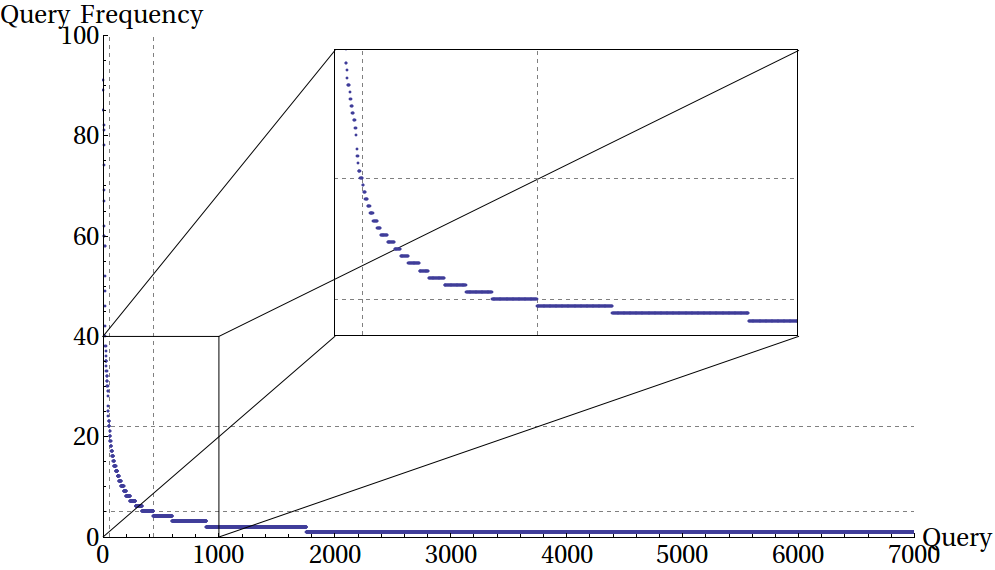
\includegraphics[scale=.3]{ecir:query-freq}
\caption{Query frequency distribution. Horizontal dashed lines represent the ``appeared 5 times" and ``appeared 22 times" thresholds when observing from bottom to top. Vertical lines divide the area under the curve in three equal parts.}
\label{fig:query-frequency}
\end{figure}

% \subsubsection{Query selection procedure} 
Out of the complete set of 15,219 user queries we select, in two steps, a subset of 50 queries to include in the study. 
First, we partition the query set into three classes: a high, mid and low frequency class. The borders of the classes are chosen so that the area under the curve in Figure \ref{fig:query-frequency} for each class is one third of the area. Queries appearing more then 22 times form the high-frequency class, between 5 and 22 form the middle-frequency class, and queries appearing less than 5 times form the low-frequency class.

Second, for each class we perform filtering. Namely, a query is skipped whenever it meets one of the following criteria: (i) it equals the title of one of the MBH recurring headings or it contains one of the words `man', `bijt', and `hond' from the series title. (ii)  it is not found in at least two of the metadata types described in Sect. \ref{sec:video-metadata-collection}. We consider the first criterion in order to exclude the non-informative queries\footnote{Queries that are expected to have a high \textit{inverse document frequency} (IDF)} and we consider the second criterion to avoid creating bias towards any metadata type. After the filtering, we are left with 12, 78, and 49 queries from the high-frequency, middle-frequency, and low-frequency class, respectively.
%\footnote{We use xapian (\url{http://xapian.org/}) IR library to implement basic search engines that index the various metadata types.}.
%We include the last criterion to avoid creating a bias in our query set towards a particular metadata type.\\
%Note that the verified \textit{Waisda?} tags were not considered as a separate metadata type from complete set of \textit{Waisda?} tags.
%In the final phase we sort the queries in each stratum on the sum of the number of videos returned by each metadata type. The count from the verified \textit{Waisda?} tags is excluded as these videos are already accounted for by the complete set of \textit{Waisda?} tags.
The top 12, top 19, and top 19 queries from the high-frequency, middle-frequency, and low-frequency class, respectively, comprise the final query set. All queries in the query set are single-term queries. This is a consequence of our second selection criterion --- the requirement of a query being present in at least two metadata types which reduces the probability of multi-term queries being selected. The second selection criterion was introduced mainly to be fair towards NCRV tags and catalog data. Our analysis of the query logs revealed that generally queries were present either in the \textit{Waisda?} tags or the captions, sometimes both. In contrast, the queries from the query logs were less frequently present in the NCRV metadata. Thus, if we omit this criterion --- and potentially include multi-term queries --- out expectation is that it will not drastically change the outcome for the \textit{Waisda?} tags and the captions. However, the NCRV metadata will likely perform worse.

\paragraph{\textbf{Relevance judgements.}}\label{sec:gold-standard}
In order to collect relevance judgements for the query set and the fragment collection we performed an on-line user experiment. To this end, we deployed a web application which was used by the participants to carry out the evaluation. %At the time of writing, the application is still up and running and it can be accessed at \url{http://tinyurl.com/c6c494v} (Dutch only).
For each participant the workflow proceeds as follows. Whenever a participant accesses the web application she is presented with a welcome page which contains a description of the task she is required to perform. Before starting with the evaluation, the participants need to fill out a questionnaire that aims at assessing their familiarity with \textit{Waisda?}, the MBH TV series and the MBH website. Then the participants proceed to the evaluation page (see Figure \ref{fig:evaluation-page}) which plays a randomly assigned fragment and lists the complete query set. During the evaluation process, the participants watch the fragment and indicate which of the concepts denoted by the queries are shown in it. \textit{We asked users to judge a fragment to be relevant for a query if it depicts the concept denoted by the query}. Each participant is asked to evaluate at least five fragments.
\begin{figure}
\centering
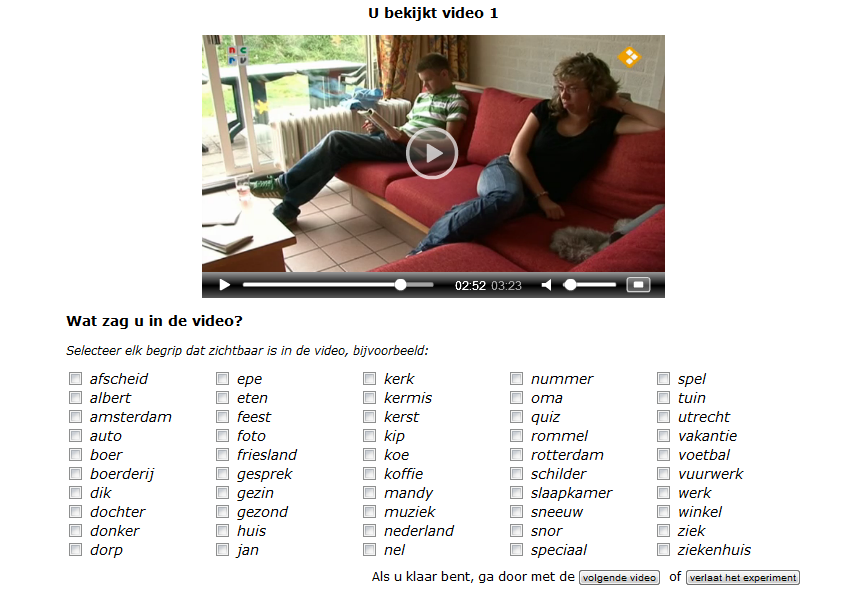
\includegraphics[scale=.5]{ecir:mendyvideo.PNG}
\caption{Screenshot of the evaluation page. At the top, a video player is placed which displays the fragment. The list of queries is rendered at the bottom.}
\label{fig:evaluation-page}
\end{figure}


\subsubsection{Participants}
The participants in the experiment were recruited mainly from the \textit{Waisda?} online community and MBH series fanbase by distributing a call for participation through the major social networking services Facebook\footnote{\url{http://www.facebook.com/}} and Twitter\footnote{\url{https://twitter.com/}}. The posted messages and tweets contained a link to our web application. 107 participants started the experiment, 83 of them evaluated at least one fragment and 25 participants evaluated more than 5 fragments. 
%Figure \ref{fig:number-of-evaluations} shows in more detail the distribution of the number of evaluated videos per participant.
Judging from the questionnaire data, the level of familiarity of participants with MBH series almost uniformly ranges from `never seen it' to `watch it regularly'. Surprisingly, the participants who never visited the MBH website or visited it only few times are the vast majority.  Also for familiarity with \textit{Waisda?}; the participants who never played or played only few times are the overwhelming majority.
%\begin{figure}
%\centering
%\includegraphics[scale=.4]{numberofevaluations.jpeg}
%\caption{Distribution of number of evaluated videos per participant.}
%\label{fig:number-of-evaluations}
%\end{figure}

\subsubsection{Participant's (Dis)agreement}
From the entire collection of 197 video fragments, 134 of them are evaluated by 2 distinct participants. The rest of the fragments, 63 in total, are evaluated by 3 distinct participants. When consolidating the relevance judgements from different participants we use majority voting; the side --- either `relevant' or `not relevant' --- that gets more votes wins. In case of a tie, we take the side of `relevant' i.e. we deem the fragment to be relevant for the query. We justify this decision with the following reasoning. The notion of relevance in our particular case is defined in terms of depiction of the concept denoted by the query in the fragment. Our queries are not abstract concepts and there is very little room for different interpretations among the participants. Thus, we believe if one participant rated  a query `not relevant' and another `relevant' for a given fragment it is most probable that the first participant simply missed it. The consolidated evaluation set is publicly available online at \url{https://goo.gl/AQcpGz}. 
The overlap among the participants in terms of evaluated videos is too small to reliably measure the inter-rater agreement with measures such as Krippendorff's alpha. However, we found that the probability of a rater rating `relevant' is 9.5\% and the probability of disagreement between raters is 10.1\%.

\section{Experiments}\label{sec:experimental-setup}
To answer the research questions formulated in Sect. \ref{sec:intro} we use a quantitative system evaluation. Namely, we implement a number of search engines and run them against the evaluation dataset described in Sect. \ref{sec:gold-standard}. In all experiments we evaluate the performance of the various search engines using the mean average precision (MAP) measure. The number of results returned by the systems is low enough (not more than 30) for the users to be willing to inspect them all. Thus, we deem that it is important that all results are good not just the top ones. This intuition is captured by MAP. To assess if the difference in performance is statistically significant we use the student's paired t-test at 0.01 level of significance as suggested by \cite{stat-sig}.

\subsection{Experiment 1}\label{sec:experiment1-setup}
In this experiment we address the first and the second research question. To this end, we retrieve fragments for the set of queries using 12 search engines. Each of the search engines utilizes the same state-of-the-art probabilistic ranking function BM25 and the only variation among them is the data they index. Consequently, differences in retrieval performance are attributed solely to the data. We implement search engines that index:

\begin{tabular}{lll}
 1. & $SE_{user}$  & all \textit{Waisda?} tags \\
 2. & $SE_{vuser}$& only verified \textit{Waisda?} tags \\
 3. & $SE_{ncrv}$& all NCRV tags \\
 4. & $SE_{catalog}$&  NCRV catalogue data \\
 5. & $SE_{caps}$& all captions\\
 6. & $SE_{caps+user}$&  all captions and all \textit{Waisda?} tags \\
 7. & $SE_{caps+catalog}$& all captions and all catalogue data \\
 8. & $SE_{ncrv+caps}$&  all captions and all NCRV tags \\
 9. & $SE_{ncrv+user}$&  all NCRV tags and all \textit{Waisda?}  tags \\
 10. & $SE_{ncrv+catalog}^{baseline}$& all NCRV tags and catalog data \\
 11. & $SE_{all-user}$&  all metadata  except  \textit{Waisda?} tags \\
 12. & $SE_{all}$&  all metadata types including  \textit{Waisda?}  tags \\
\end{tabular}

\noindent
$SE_{ncrv+catalog}^{baseline}$ is an approximation of the search functionality offered on the web site dedicated to MBH series. We use it as a baseline for comparing the search performance of the other search engines. By comparing the performance of $SE_{user}$ and $SE_{vuser}$ we are able to see if using all tags as opposed to only verified tags is detrimental or beneficial for fragment search (\textit{RQ2}). Furthermore, comparing the performance of $SE_{user}$ and systems 3 through 12 will reveal how well user tags are doing --- on their own and in combination --- compared to other types of metadata (\textit{RQ1}).

%\subsubsection{Experiment 2}
%The goal of this experiment is to answer the third research question. Once again, we retrieve fragments using the $SE_{user}$, $SE_{vuser}$,  $SE_{ncrv}$, $SE_{catalog}$, and $SE_{subs}$ search engines from the previous experiment. However, this time we consider several query subsets, where each subset contains queries classified in specific category of the Panofsky-Shatford model. By comparing the performance of the search engines across difference categories of the Panofsky-Shatford model we will see for which type(s) of queries user tags are best suited.

\subsection{Experiment 2} \label{sec:experiment2-setup}
In this experiment we address the third research question. We retrieve fragments for the set of queries using two collections of search engines. The first collection consists of search engines that index snapshots\footnote{A snapshot contains all user tags up to a given point in time.} of all user tags taken periodically once a week. Identically, the second collection consists of search engines that index snapshots of the verified tags taken at the same time points as the snapshots from the first collection. As with experiment 1, all search engines use the same probabilistic ranking function BM25 and the only variation among them is the data that they index. Examining the performance of search engines within a collection reveals how tag search performance changes over time. By examining the performance of search engines across collections we learn how all tags perform compared to verified tags.

\section{Results}\label{sec:results}
In this section we present the results of our experiments.
\subsection{Experiment 1}
The results for this experiment are summarized in Table \ref{table:results}. As seen, considering only verified tags yields worse search performance than considering all tags. Intuitively, verified tags should yield higher precision but lower recall than all tags. Indeed, the average search precision of verified tags (0.59) across the queries is higher than the average search precision of all tags (0.49). However, search based on all tags yields more relevant results --- the average search recall of all tags (0.42) is higher than the averages search recall of the verified tags (0.28). In fact, for 35 queries the non-verified tags yielded relevant results ---on average 4---not found by verified tags\footnote{More detailed figures can be found the Appendix \ref{appen:prec-recall} at the end of the thesis.}. It seems the \textit{tag verification} criterion is too conservative in a sense that it filters out tags that are in fact useful for search.

Search based on user tags ($SE_{user}$) significantly outperforms search based on other metadata types alone. Indeed, search based on user tags is approximately 69\% more successful than search based on the in-house NCRV tags ($SE_{ncrv}$). We believe this is attributed to the fact that NCRV tags are relatively scarce and cover mainly prevalent topics. In this sense, user tags are complementary to the NCRV tags and the combination of both is mutually beneficial. Indeed, the search engine that indexes both user tags and NCRV tags, $S_{ncrv+user}$, yields a performance increase of 20\% and 90\% over search engines $S_{user}$ and $S_{ncrv}$, respectively.\\
Furthermore, search based on solely on user tags yields better performance from our baseline search engine, $SE_{ncrv+catalog}^{baseline}$. Indeed, the MAP scores of $S_{user}$ and $SE_{ncrv+catalog}^{baseline}$ indicate a performance increase of 46\%.\\
Comparison of the MAP scores of $SE_{user}$ and $SE_{caps}$ indicates that user tags outperform captions by approximately 39\%. This can be explained by the fact that captions only cover the audio portion of the video content, whereas user tags cover both audio and visual. In fact, previous work \cite{kcap} suggested that players tend to describe more things that appear visually in a video. Combination of captions and user tags proves to be beneficial: $SE_{caps+user}$ outperforms $SE_{caps}$ and $S_{user}$ by 64\% and 13\%, respectively.\\
Lastly, the search engine that indexes all available types of metadata, $SE_{all}$, performs best. This is to a large extend due to the contribution of user tags. Indeed, $SE_{all}$ outperforms the search engine that indexes all metadata types except for user tags, $SE_{all-user}$, by 33\%. Obviously, the said difference can only be attributed to the effect of the user tags. Interestingly, search based on user tags alone outperforms by 5\%  $SE_{all-user}$, which is the best performing search engine that does not index user tags.

\begin{table}[tb]
\centering
\begin{footnotesize}
\label{table:results}
\begin{tabular}{l|l|l|l}
\toprule
$SE_{user}$ & $SE_{vuser}$ & $SE_{ncrv}$ & $SE_{catalog}$\\
\hline
$0.219^{\approx \uparrow}$ & $0.143^{\downarrow \approx}$ & $0.138^{\downarrow \downarrow}$ & $0.077^{\downarrow \downarrow}$\\
\hline
\multicolumn{4}{c}{ }\\
\hline
$SE_{caps}$ & $SE_{caps+user}$ & $SE_{caps+catalog}$ & $SE_{ncrv+caps}$\\
\hline
$0.157^{\downarrow \uparrow}$ & $0.247^{\uparrow \uparrow}$ & $0.183^{\downarrow \uparrow}$ & $0.201^{\downarrow \uparrow}$ \\
\hline
\multicolumn{4}{c}{ }\\
\hline
$SE_{ncrv+user}$ & $SE_{ncrv+catalog}^{baseline}$ & $SE_{all-user}$ & $SE_{all}$\\
\hline
$0.263^{\uparrow \uparrow}$ & $0.150^{\downarrow \uparrow}$ & $0.208^{\downarrow \uparrow}$ & $0.276^{\uparrow \uparrow}$ \\
\bottomrule
\end{tabular}
\caption{Results for experiment 1: MAP scores for the search engines --- MAP score for given search engine is given immediately bellow. $\uparrow$, $\downarrow$, and $\approx$ indicate if a score is significantly better, worse, or statistically indistinguishable from the MAP scores of $SE_{user}$ and $SE_{vuser}$, in that order.}
\end{footnotesize}
\end{table}


%\begin{table}[tb]
%\centering
%\begin{footnotesize}
%\begin{tabular}{cl|r|r|r|r|r}
%\toprule
%  & \multicolumn{5}{c}{\textbf{Query set}}\\
% \cline{3-7}
%& & \textit{All} & \textit{A-What} & \textit{G-What} & \textit{G-Where} & \textit{G-Who}   \\
%\cline{2-7}
%\multirow{1}{*}{\rotatebox{90}{\textbf{Search engine}}}&\multicolumn{1}{|l|}{$SE_{user}$}& $0.219^{\approx \uparrow}$ &  &  &  &  \\ 
%\cline{2-7}
% & \multicolumn{1}{|l|}{$SE_{vuser}$} & $0.143^{\downarrow \approx}$\\
% \cline{2-7}
% & \multicolumn{1}{|l|}{$SE_{ncrv}$} & $0.138^{\downarrow \downarrow}$\\
% \cline{2-7}
% & \multicolumn{1}{|l|}{$SE_{catalog}$}& $0.077^{\downarrow \downarrow}$\\
% \cline{2-7}
% & \multicolumn{1}{|l|}{$SE_{subs}$} & $0.157^{\downarrow \uparrow}$ \\
%  \cline{2-7}
% & \multicolumn{1}{|l|}{$SE_{subs+user}$}&  $0.247^{\uparrow \uparrow}$\\
%  \cline{2-7}
% & \multicolumn{1}{|l|}{$SE_{subs+catalog}$}&  $0.183^{\downarrow \uparrow}$\\
%  \cline{2-7}
% & \multicolumn{1}{|l|}{$SE_{ncrv+subs}$}&  $0.201^{\downarrow \uparrow}$\\
%  \cline{2-7}
% & \multicolumn{1}{|l|}{$SE_{ncrv+user}$}& $0.263^{\uparrow \uparrow}$\\
%  \cline{2-7}
% & \multicolumn{1}{|l|}{$SE_{ncrv+catalog}^{baseline}$}& $0.150^{\downarrow \uparrow}$\\
%  \cline{2-7}
% & \multicolumn{1}{|l|}{$SE_{all-user}$} & $0.208^{\downarrow \uparrow}$\\
%  \cline{2-7}
% & \multicolumn{1}{|l|}{$SE_{all}$} & $0.276^{\uparrow \uparrow}$
%
%\bottomrule
%\end{tabular*}
%\end{footnotesize}
%\caption{Results for experiment 1 and experiment 2: MAP scores for several query sets and 8 search engines. $\uparrow$, $\downarrow$, and $\approx$ indicate if a score is significantly better, worse, or statistically indistinguishable from the MAP scores of $SE_{user}$ and $SE_{vuser}$, in that order.}
%\label{table:results}
%\end{table}

%\subsection{Experiment 2}

\subsubsection{Analysis of False Positives}
One of the conclusions drawn above is that the precision of $SE_{user}$ ---or in other words when considering all user tags --- is relatively low. In order to get a better insight into the reasons that lead to poor precision we manually analysed a sample of the false positives\footnote{A search result is a false positive if it is returned by $SE_{user}$ but was deemed `not relevant' by our evaluators.} among the results obtained from $SE_{user}$ . Note that given the definition of search precision, it is the false positives that are accountable for the drop in the precision score.

In the course of the analysis, we randomly picked fifteen queries from the query set and investigated the false positives retrieved for them --- 192 in total. For each query-fragment pair we watched 10 seconds prior and 10 seconds after the point when the tag that matched the query was entered. The occurrence of the query instance in the fragment is then classified as either `visual', `nonvisual' based on the same criterion used by the evaluators, or \textit{unrelated}. The \textit{unrelated} category consists of tags that are not describing the content of the video and can be accounted as errors by the users. The `visual' class is further subdivided into the following disjoint subclasses which designate how/where the instance denoted by the query is depicted along the spatial and temporal dimensions:
\begin{itemize}
\item \textit{Intro}. The instance is in the opening segment of the fragment which is usually unrelated with the rest of the fragment.
\item \textit{Short-lived in background}. The instance appears for a brief moment, e.g. less than a second, in the background and not in opening segment. An example of this would be a \textit{car} passing by in the background.
\item \textit{Short-lived in foreground}. The instance appears for a brief moment, e.g. less than a second, in the foreground and not in opening segment. An example of this  would be a \textit{person} passing by in front of the camera.
\item \textit{Long-lived}. The instance appears either in the background or in the foreground for a longer period of time.
\end{itemize}
The `nonvisual' class is subdivided into the following disjoint subclasses:
\begin{itemize}
\item \textit{Captions in intro}. The instance appears only in captions in the opening segment.
\item \textit{Captions}. The instance appears only in captions and not in the opening segment.
\item \textit{Screen text}. Screen text referring to the instance.
\end{itemize}
The results of the classification are summarized in Table \ref{tab:exp1-false-pos}. As seen, significant fraction of the false positives were caused from tags associated with the opening segments: 17\% of them refer to visual instances and 12\% are mentioned in the captions in the opening fragment. Moreover, 15\% of the false positives are a result of the tags found only in the captions not in the opening segments. In general, it is context-dependent whether these cases should be considered relevant or not. In this analysis, we deemed visual appearances in opening segments as relevant and references in captions as not relevant due to our interpretation of (visual) relevance. However, in other scenarios the interpretation of relevance may differ. Nevertheless, it is straightforward to detect these cases automatically and include/exclude them as input for search depending on the context.
The \textit{short-lived background/foreground} and \textit{other} cases were most likely missed by the evaluators. Had they been correctly identified the outcome of the comparison given above would have been even more favourable for \textit{Waisda?} tags. 
Furthermore, 20\% of the false positives were visual appearances of long-lived instances i.e. objects appearing on screen for a longer period of time. However, it is interesting to mention that these cases usually involved ambiguity and the context and the hints provided by the current or the previous scenes from the video were required to make the correct interpretation. For example, for the query \textit{boer} (the Dutch word for \textit{farmer}) there were instances where a person while being a farmer, a fact established in the previous scenes, in one particular scene was not in the typical farmer's attire and could not be identified as such using only the information provided on the screen. It is easy to imagine how a tagger having seen the video from the beginning and having this extended context could interpret the person as a farmer. Needless to say, what is the right answer in these cases depends on the particular application context. Finally, 21\% of the false positives were caused by incorrect tags not at all related with the content of the fragments.

\begin{table}[tb]
\centering
\begin{footnotesize}
\begin{tabular*}{\columnwidth}{@{\extracolsep{\fill}}lrr}
\toprule
\multirow{4}{*}{\textbf{Visual}} & \textit{Intro}  \T \B & 33 (17\%) \\
  %\cline{2-3}
 & \textit{Short-lived in background} \T \B & 13 (7\%)\\
 & \textit{Short-lived in foreground} \B &  15 (8\%)\\
 & \textit{Long-lived} \B & 38 (20\%)\\
\hline
\multirow{4}{*}{\textbf{Nonvisual}} & \textit{Captions in intro} \B \T & 23 (12\%)\\
%\cline{2-3}
 & \textit{Captions} \T \B &  28 (15\%)\\
 & \textit{Screen text} \B & 1 (0\%)\\
 \hline
 &&\\
 \textbf{Unrelated} & &  41 (21\%) \\
 &&\\
\bottomrule
\end{tabular*}
\end{footnotesize}
\caption{Experiment 1 false positives classification.}
\label{tab:exp1-false-pos}
\end{table}


\subsection{Experiment 2}\label{ecir:over-time-results}
In this section we present the results from our second experiment which addresses the third research question. Figure \ref{fig:snapshop-map} shows the MAP scores of the search engines indexing the weekly snapshots of all tags and only the verified tags. Figure \ref{fig:snapshot-tcount}, on the other hand, shows how the number of all tags and verified tags increased over time.
Looking at Figure \ref{fig:snapshop-map} we conclude that most of the time the search performance for both the verified tags and all tags is monotonically increasing with the number of tags. In other words, the more tags we amass, the better our effectiveness in searching fragments becomes. Furthermore, looking at the pairwise search performance differences between the search engines that index the weekly snapshots of all tags and verified tags (vertical dashed lines between plots in Figure \ref{fig:snapshop-map}), we conclude that using all tags for search opposed to only verified ones yields consistently better results. In fact, search performance improvements are statistically significant for every single pair.

The performance of search based on all user tags surpasses our baseline, $SE_{ncrv+catalog}^{baseline}$, around the $11^{th}$ week after 42,271 tags have been collected (Figure \ref{fig:snapshot-tcount}). Beyond that point the said difference in performance steadily increases as more tags are collected. With $SE_{all-user}$, which is the best performing search engine that does not index user tags, this happens a bit later. In particular, after the $18^{th}$ week and 91,508 collected tags, $SE_{user}$ starts to outperform $SE_{all-user}$. Thus, there is a point somewhere between the $18^{th}$ and $19^{th}$ week when the collected user tags outperform all search engines that do not index tags.

It is also interesting to note that the precision and recall of search based on all tags are monotonically non-decreasing with the number of tags for each query in our set. The results for search precision and recall can be found in the appendices \ref{appen:precovertime} and \ref{appen:recovertime} at the end of the thesis, respectively.

\begin{figure}
\subfigure[The MAP scores of the user tags over time. Horizontal lines represent MAP scores of $SE_{ncrv+catalog}^{baseline}$ and $SE_{all-user}$]{
	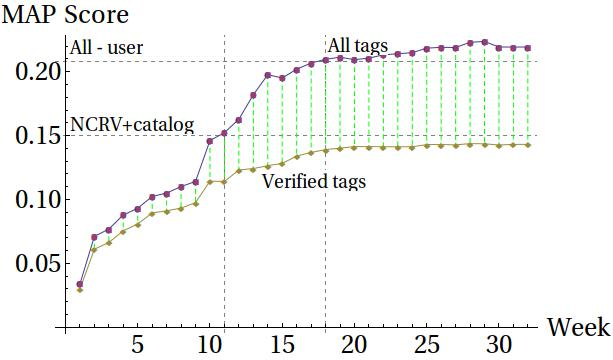
\includegraphics[scale=.28]{ecir:snapshots-map.jpeg}
	\label{fig:snapshop-map}
}
\subfigure[The total number of tags over time]{
	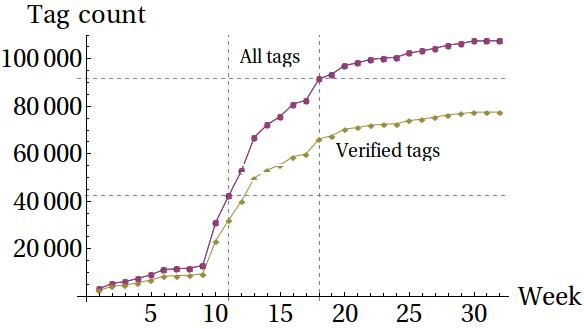
\includegraphics[scale=.3]{ecir:snapshots-tag-count.jpeg}
	\label{fig:snapshot-tcount}
}
\caption{MAP scores and tag count over time.}
\end{figure}

\section{Conclusions and Future Work}\label{sec:conclusions}
In this paper we have studied the added value of user tags for video search. For this reason we have created a publicly available evaluation dataset that consists of real-life user queries, a video fragment collection, and relevance judgements. 

Search based solely on user tags outperforms search based on other types of metadata such as in-house (NCRV) tags or captions. Thus if any of the other metadata types are unavailable or costly to acquire, relying only on sufficient user tags for search could yield equal or even better results. In our dataset, combining user tags with other metadata types is beneficial for search. In fact, the search engine that exploits all available metadata performs best, to large part due to the contribution of the user tags---the observed performance improvement is 33\%. 

Exploiting only verified user tags for search gives poorer performance than search based on all user tags. While search based on verified tags yields higher precision, it also has lower recall compared to all user tags. In fact, for most of the queries non-verified tags provided relevant results that were not found by the verified tags. This proves that considering only verified tags is too conservative filtering criterion resulting in discarding non-verified user tags that are valid video descriptors and thus useful for search. 

Search performance steadily increases as more user tags are collected. This is true for both verified and all tags. Moreover, search based on all tags consistently outperforms search based only on verified tags. When the average number of tags is slightly more than 2 tags per second, the search using all tags outperforms all search engines that are not indexing user tags. Such an estimate could be used as an indicator whether a video has been tagged enough.

In the future, we will study whether certain tag features such as reputation of the tag author and provenance can be used to detect and exclude non-useful non-verified tags thereby increasing the search precision without sacrificing the recall. 
